\documentclass[twoside]{book}

% Packages required by doxygen
\usepackage{fixltx2e}
\usepackage{calc}
\usepackage{doxygen}
\usepackage[export]{adjustbox} % also loads graphicx
\usepackage{graphicx}
\usepackage[utf8]{inputenc}
\usepackage{makeidx}
\usepackage{multicol}
\usepackage{multirow}
\PassOptionsToPackage{warn}{textcomp}
\usepackage{textcomp}
\usepackage[nointegrals]{wasysym}
\usepackage[table]{xcolor}

% Font selection
\usepackage[T1]{fontenc}
\usepackage[scaled=.90]{helvet}
\usepackage{courier}
\usepackage{amssymb}
\usepackage{sectsty}
\renewcommand{\familydefault}{\sfdefault}
\allsectionsfont{%
  \fontseries{bc}\selectfont%
  \color{darkgray}%
}
\renewcommand{\DoxyLabelFont}{%
  \fontseries{bc}\selectfont%
  \color{darkgray}%
}
\newcommand{\+}{\discretionary{\mbox{\scriptsize$\hookleftarrow$}}{}{}}

% Page & text layout
\usepackage{geometry}
\geometry{%
  a4paper,%
  top=2.5cm,%
  bottom=2.5cm,%
  left=2.5cm,%
  right=2.5cm%
}
\tolerance=750
\hfuzz=15pt
\hbadness=750
\setlength{\emergencystretch}{15pt}
\setlength{\parindent}{0cm}
\setlength{\parskip}{0.2cm}
\makeatletter
\renewcommand{\paragraph}{%
  \@startsection{paragraph}{4}{0ex}{-1.0ex}{1.0ex}{%
    \normalfont\normalsize\bfseries\SS@parafont%
  }%
}
\renewcommand{\subparagraph}{%
  \@startsection{subparagraph}{5}{0ex}{-1.0ex}{1.0ex}{%
    \normalfont\normalsize\bfseries\SS@subparafont%
  }%
}
\makeatother

% Headers & footers
\usepackage{fancyhdr}
\pagestyle{fancyplain}
\fancyhead[LE]{\fancyplain{}{\bfseries\thepage}}
\fancyhead[CE]{\fancyplain{}{}}
\fancyhead[RE]{\fancyplain{}{\bfseries\leftmark}}
\fancyhead[LO]{\fancyplain{}{\bfseries\rightmark}}
\fancyhead[CO]{\fancyplain{}{}}
\fancyhead[RO]{\fancyplain{}{\bfseries\thepage}}
\fancyfoot[LE]{\fancyplain{}{}}
\fancyfoot[CE]{\fancyplain{}{}}
\fancyfoot[RE]{\fancyplain{}{\bfseries\scriptsize Generated on Mon Oct 5 2015 13\+:16\+:57 for N3 by Doxygen }}
\fancyfoot[LO]{\fancyplain{}{\bfseries\scriptsize Generated on Mon Oct 5 2015 13\+:16\+:57 for N3 by Doxygen }}
\fancyfoot[CO]{\fancyplain{}{}}
\fancyfoot[RO]{\fancyplain{}{}}
\renewcommand{\footrulewidth}{0.4pt}
\renewcommand{\chaptermark}[1]{%
  \markboth{#1}{}%
}
\renewcommand{\sectionmark}[1]{%
  \markright{\thesection\ #1}%
}

% Indices & bibliography
\usepackage{natbib}
\usepackage[titles]{tocloft}
\setcounter{tocdepth}{3}
\setcounter{secnumdepth}{5}
\makeindex

% Hyperlinks (required, but should be loaded last)
\usepackage{ifpdf}
\ifpdf
  \usepackage[pdftex,pagebackref=true]{hyperref}
\else
  \usepackage[ps2pdf,pagebackref=true]{hyperref}
\fi
\hypersetup{%
  colorlinks=true,%
  linkcolor=blue,%
  citecolor=blue,%
  unicode%
}

% Custom commands
\newcommand{\clearemptydoublepage}{%
  \newpage{\pagestyle{empty}\cleardoublepage}%
}


%===== C O N T E N T S =====

\begin{document}

% Titlepage & ToC
\hypersetup{pageanchor=false,
             bookmarks=true,
             bookmarksnumbered=true,
             pdfencoding=unicode
            }
\pagenumbering{roman}
\begin{titlepage}
\vspace*{7cm}
\begin{center}%
{\Large N3 }\\
\vspace*{1cm}
{\large Generated by Doxygen 1.8.10}\\
\vspace*{0.5cm}
{\small Mon Oct 5 2015 13:16:57}\\
\end{center}
\end{titlepage}
\clearemptydoublepage
\tableofcontents
\clearemptydoublepage
\pagenumbering{arabic}
\hypersetup{pageanchor=true}

%--- Begin generated contents ---
\chapter{Hierarchical Index}
\section{Class Hierarchy}
This inheritance list is sorted roughly, but not completely, alphabetically\+:\begin{DoxyCompactList}
\item N\+S\+Object\begin{DoxyCompactList}
\item \contentsline{section}{Arvore}{\pageref{interface_arvore}}{}
\begin{DoxyCompactList}
\item \contentsline{section}{Arvore\+Frutifera}{\pageref{interface_arvore_frutifera}}{}
\begin{DoxyCompactList}
\item \contentsline{section}{Laranjeira}{\pageref{interface_laranjeira}}{}
\item \contentsline{section}{Limoeiro}{\pageref{interface_limoeiro}}{}
\end{DoxyCompactList}
\end{DoxyCompactList}
\item \contentsline{section}{Bosque}{\pageref{interface_bosque}}{}
\item \contentsline{section}{Fruta}{\pageref{interface_fruta}}{}
\end{DoxyCompactList}
\end{DoxyCompactList}

\chapter{Class Index}
\section{Class List}
Here are the classes, structs, unions and interfaces with brief descriptions\+:\begin{DoxyCompactList}
\item\contentsline{section}{\hyperlink{interface_arvore}{Arvore} \\*Classe que representa uma árvore }{\pageref{interface_arvore}}{}
\item\contentsline{section}{\hyperlink{interface_arvore_frutifera}{Arvore\+Frutifera} \\*Classe que representa uma árvore frutífera }{\pageref{interface_arvore_frutifera}}{}
\item\contentsline{section}{\hyperlink{interface_bosque}{Bosque} \\*Classe que representa um bosque e suas árvores }{\pageref{interface_bosque}}{}
\item\contentsline{section}{\hyperlink{interface_fruta}{Fruta} \\*Classe que representa uma fruta }{\pageref{interface_fruta}}{}
\item\contentsline{section}{\hyperlink{interface_laranjeira}{Laranjeira} \\*Classe que representa uma laranjeira }{\pageref{interface_laranjeira}}{}
\item\contentsline{section}{\hyperlink{interface_limoeiro}{Limoeiro} \\*Classe que representa uma limoeira }{\pageref{interface_limoeiro}}{}
\end{DoxyCompactList}

\chapter{File Index}
\section{File List}
Here is a list of all files with brief descriptions\+:\begin{DoxyCompactList}
\item\contentsline{section}{\hyperlink{_arvore_8h}{Arvore.\+h} }{\pageref{_arvore_8h}}{}
\item\contentsline{section}{\hyperlink{_arvore_8m}{Arvore.\+m} }{\pageref{_arvore_8m}}{}
\item\contentsline{section}{\hyperlink{_arvore_frutifera_8h}{Arvore\+Frutifera.\+h} }{\pageref{_arvore_frutifera_8h}}{}
\item\contentsline{section}{\hyperlink{_arvore_frutifera_8m}{Arvore\+Frutifera.\+m} }{\pageref{_arvore_frutifera_8m}}{}
\item\contentsline{section}{\hyperlink{_bosque_8h}{Bosque.\+h} }{\pageref{_bosque_8h}}{}
\item\contentsline{section}{\hyperlink{_bosque_8m}{Bosque.\+m} }{\pageref{_bosque_8m}}{}
\item\contentsline{section}{\hyperlink{_fruta_8h}{Fruta.\+h} }{\pageref{_fruta_8h}}{}
\item\contentsline{section}{\hyperlink{_fruta_8m}{Fruta.\+m} }{\pageref{_fruta_8m}}{}
\item\contentsline{section}{\hyperlink{_laranjeira_8h}{Laranjeira.\+h} }{\pageref{_laranjeira_8h}}{}
\item\contentsline{section}{\hyperlink{_laranjeira_8m}{Laranjeira.\+m} }{\pageref{_laranjeira_8m}}{}
\item\contentsline{section}{\hyperlink{_limoeiro_8h}{Limoeiro.\+h} }{\pageref{_limoeiro_8h}}{}
\item\contentsline{section}{\hyperlink{_limoeiro_8m}{Limoeiro.\+m} }{\pageref{_limoeiro_8m}}{}
\item\contentsline{section}{\hyperlink{main_8m}{main.\+m} }{\pageref{main_8m}}{}
\end{DoxyCompactList}

\chapter{Class Documentation}
\hypertarget{interface_arvore}{}\section{Arvore Class Reference}
\label{interface_arvore}\index{Arvore@{Arvore}}


Classe que representa uma árvore.  




{\ttfamily \#import $<$Arvore.\+h$>$}

Inheritance diagram for Arvore\+:\begin{figure}[H]
\begin{center}
\leavevmode
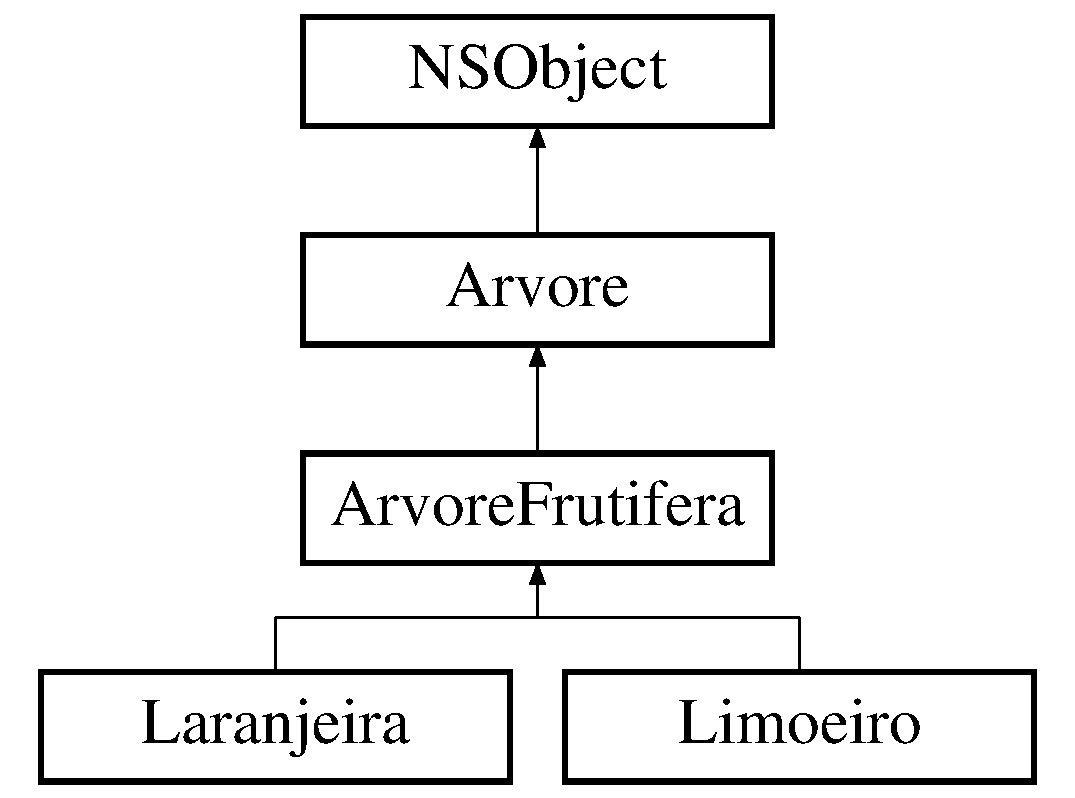
\includegraphics[height=4.000000cm]{interface_arvore}
\end{center}
\end{figure}
\subsection*{Instance Methods}
\begin{DoxyCompactItemize}
\item 
(N\+S\+String $\ast$) -\/ \hyperlink{interface_arvore_a660cb6ff62fd1d1a42113af3cb5ec55e}{get\+Nome\+Popular}
\item 
(N\+S\+String $\ast$) -\/ \hyperlink{interface_arvore_a2316550aad9b4ccb9ce44ce28c17f84c}{get\+Nome\+Cientifico}
\item 
(void) -\/ \hyperlink{interface_arvore_afd29b615282d878986e2ba7e66fc0255}{append\+Anotacao\+:dia\+:}
\begin{DoxyCompactList}\small\item\em Adiciona anotação no dia passado. \end{DoxyCompactList}\end{DoxyCompactItemize}
\subsection*{Protected Attributes}
\begin{DoxyCompactItemize}
\item 
N\+S\+String $\ast$ \hyperlink{interface_arvore_aa80507632b6a530535acd684f8396c59}{nome\+Cientifico}
\begin{DoxyCompactList}\small\item\em Nome científico da árvore. \end{DoxyCompactList}\item 
N\+S\+String $\ast$ \hyperlink{interface_arvore_a4514f27ae9acb812d6b28c4efa625807}{nome\+Popular}
\begin{DoxyCompactList}\small\item\em Nome popular da árvore. \end{DoxyCompactList}\item 
N\+S\+Mutable\+String $\ast$ \hyperlink{interface_arvore_a643c6f5a0e0756823ef781b06d3aeba4}{anotacoes}
\begin{DoxyCompactList}\small\item\em Anotações feitas sobre a árvore, organizadas por dia. \end{DoxyCompactList}\end{DoxyCompactItemize}


\subsection{Detailed Description}
Classe que representa uma árvore. 

\subsection{Method Documentation}
\hypertarget{interface_arvore_afd29b615282d878986e2ba7e66fc0255}{}\index{Arvore@{Arvore}!append\+Anotacao\+:dia\+:@{append\+Anotacao\+:dia\+:}}
\index{append\+Anotacao\+:dia\+:@{append\+Anotacao\+:dia\+:}!Arvore@{Arvore}}
\subsubsection[{append\+Anotacao\+:dia\+:(\+N\+S\+String $\ast$nova\+Anotacao,[dia] int dia)}]{\setlength{\rightskip}{0pt plus 5cm}-\/ (void) append\+Anotacao\+: 
\begin{DoxyParamCaption}
\item[{(N\+S\+String$\ast$)}]{nova\+Anotacao}
\item[{dia:(int)}]{dia}
\end{DoxyParamCaption}
}\label{interface_arvore_afd29b615282d878986e2ba7e66fc0255}


Adiciona anotação no dia passado. 


\begin{DoxyParams}{Parameters}
{\em nova\+Anotacao} & \\
\hline
{\em dia} & \\
\hline
\end{DoxyParams}
\hypertarget{interface_arvore_a2316550aad9b4ccb9ce44ce28c17f84c}{}\index{Arvore@{Arvore}!get\+Nome\+Cientifico@{get\+Nome\+Cientifico}}
\index{get\+Nome\+Cientifico@{get\+Nome\+Cientifico}!Arvore@{Arvore}}
\subsubsection[{get\+Nome\+Cientifico()}]{\setlength{\rightskip}{0pt plus 5cm}-\/ (N\+S\+String $\ast$) get\+Nome\+Cientifico 
\begin{DoxyParamCaption}
{}
\end{DoxyParamCaption}
}\label{interface_arvore_a2316550aad9b4ccb9ce44ce28c17f84c}
\begin{DoxyReturn}{Returns}
Retorna o nome científico da árvore. 
\end{DoxyReturn}
\hypertarget{interface_arvore_a660cb6ff62fd1d1a42113af3cb5ec55e}{}\index{Arvore@{Arvore}!get\+Nome\+Popular@{get\+Nome\+Popular}}
\index{get\+Nome\+Popular@{get\+Nome\+Popular}!Arvore@{Arvore}}
\subsubsection[{get\+Nome\+Popular()}]{\setlength{\rightskip}{0pt plus 5cm}-\/ (N\+S\+String $\ast$) get\+Nome\+Popular 
\begin{DoxyParamCaption}
{}
\end{DoxyParamCaption}
}\label{interface_arvore_a660cb6ff62fd1d1a42113af3cb5ec55e}
\begin{DoxyReturn}{Returns}
Retorna o nome popular da árvore. 
\end{DoxyReturn}


\subsection{Member Data Documentation}
\hypertarget{interface_arvore_a643c6f5a0e0756823ef781b06d3aeba4}{}\index{Arvore@{Arvore}!anotacoes@{anotacoes}}
\index{anotacoes@{anotacoes}!Arvore@{Arvore}}
\subsubsection[{anotacoes}]{\setlength{\rightskip}{0pt plus 5cm}-\/ (N\+S\+Mutable\+String$\ast$) anotacoes\hspace{0.3cm}{\ttfamily [protected]}}\label{interface_arvore_a643c6f5a0e0756823ef781b06d3aeba4}


Anotações feitas sobre a árvore, organizadas por dia. 

\hypertarget{interface_arvore_aa80507632b6a530535acd684f8396c59}{}\index{Arvore@{Arvore}!nome\+Cientifico@{nome\+Cientifico}}
\index{nome\+Cientifico@{nome\+Cientifico}!Arvore@{Arvore}}
\subsubsection[{nome\+Cientifico}]{\setlength{\rightskip}{0pt plus 5cm}-\/ (N\+S\+String$\ast$) nome\+Cientifico\hspace{0.3cm}{\ttfamily [protected]}}\label{interface_arvore_aa80507632b6a530535acd684f8396c59}


Nome científico da árvore. 

\hypertarget{interface_arvore_a4514f27ae9acb812d6b28c4efa625807}{}\index{Arvore@{Arvore}!nome\+Popular@{nome\+Popular}}
\index{nome\+Popular@{nome\+Popular}!Arvore@{Arvore}}
\subsubsection[{nome\+Popular}]{\setlength{\rightskip}{0pt plus 5cm}-\/ (N\+S\+String$\ast$) nome\+Popular\hspace{0.3cm}{\ttfamily [protected]}}\label{interface_arvore_a4514f27ae9acb812d6b28c4efa625807}


Nome popular da árvore. 



The documentation for this class was generated from the following files\+:\begin{DoxyCompactItemize}
\item 
\hyperlink{_arvore_8h}{Arvore.\+h}\item 
\hyperlink{_arvore_8m}{Arvore.\+m}\end{DoxyCompactItemize}

\hypertarget{interface_arvore_frutifera}{}\section{Arvore\+Frutifera Class Reference}
\label{interface_arvore_frutifera}\index{Arvore\+Frutifera@{Arvore\+Frutifera}}


Classe que representa uma árvore frutífera.  




{\ttfamily \#import $<$Arvore\+Frutifera.\+h$>$}

Inheritance diagram for Arvore\+Frutifera\+:\begin{figure}[H]
\begin{center}
\leavevmode
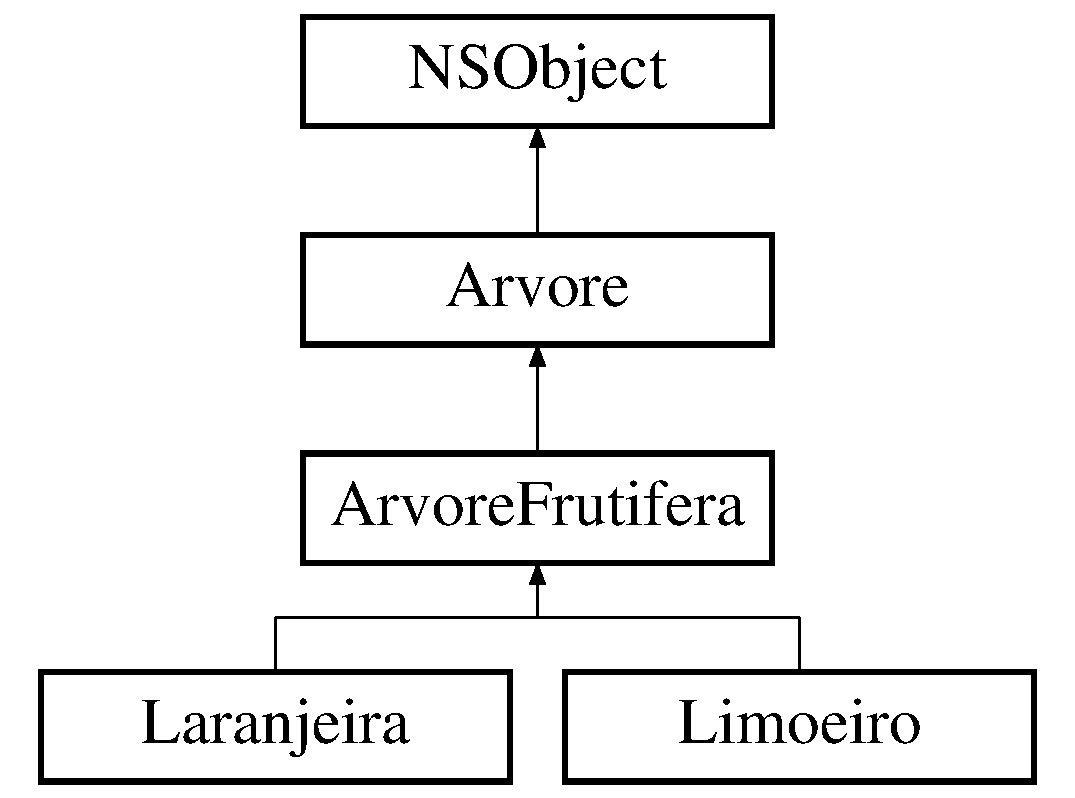
\includegraphics[height=4.000000cm]{interface_arvore_frutifera}
\end{center}
\end{figure}
\subsection*{Instance Methods}
\begin{DoxyCompactItemize}
\item 
(int) -\/ \hyperlink{interface_arvore_frutifera_a691238edae60caa881896cb35691c653}{get\+Quantidade\+Frutas}
\item 
(void) -\/ \hyperlink{interface_arvore_frutifera_ac1e9d292fe4f2bbdc047bee97527426d}{set\+Quantidade\+Frutas\+:}
\begin{DoxyCompactList}\small\item\em Seta a quantidade média de frutas que a árvore possuía na hora da análise. \end{DoxyCompactList}\item 
(char $\ast$) -\/ \hyperlink{interface_arvore_frutifera_a8f487349ee1aa0bdb6871d1685c16843}{get\+Epoca\+Frutifera}
\item 
(void) -\/ \hyperlink{interface_arvore_frutifera_a0e2af9007f8174001ce9cbc4d92d2549}{add\+Fruta\+:}
\begin{DoxyCompactList}\small\item\em Adiciona fruta na lista de frutas analisadas. \end{DoxyCompactList}\item 
(void) -\/ \hyperlink{interface_arvore_frutifera_a6a388570a869639f60432a106c1b0e46}{insert\+Fruta\+:posicao\+:}
\begin{DoxyCompactList}\small\item\em Adiciona fruta na lista de frutas analisadas na posição passada. \end{DoxyCompactList}\item 
(\hyperlink{interface_fruta}{Fruta} $\ast$) -\/ \hyperlink{interface_arvore_frutifera_a5628e0fc6b0d5b8b006dfe3d405e4584}{fruta\+At\+Index\+:}
\item 
(void) -\/ \hyperlink{interface_arvore_frutifera_a00ebdbd08305303aa49fcac8655e8a54}{remove\+Fruta\+At\+Index\+:}
\begin{DoxyCompactList}\small\item\em Remove fruta que se encontra na posição passada. \end{DoxyCompactList}\item 
(B\+O\+O\+L) -\/ \hyperlink{interface_arvore_frutifera_abe74166806547db2cf256220a5fd3a37}{is\+Arvore\+Frutifera\+:}
\end{DoxyCompactItemize}
\subsection*{Protected Attributes}
\begin{DoxyCompactItemize}
\item 
char $\ast$ \hyperlink{interface_arvore_frutifera_a0e22588b833e760b868e05dc2e3c7af9}{epoca\+Frutifera}
\begin{DoxyCompactList}\small\item\em String com o nome da estação frutífera. \end{DoxyCompactList}\item 
int $\ast$ \hyperlink{interface_arvore_frutifera_aa0f26437071d5fc42bb990c9c49906be}{quantidade\+Frutas}
\begin{DoxyCompactList}\small\item\em Inteiro indicando a quantidade de frutas vistas na árvore (média). \end{DoxyCompactList}\item 
N\+S\+Mutable\+Array$<$ \hyperlink{interface_fruta}{Fruta} $\ast$ $>$ $\ast$ \hyperlink{interface_arvore_frutifera_ae837cbe18a17ea2d500517ab72ce818f}{frutas\+Analisadas}
\begin{DoxyCompactList}\small\item\em Lista de frutas que foram analisadas desta árvore. \end{DoxyCompactList}\end{DoxyCompactItemize}


\subsection{Detailed Description}
Classe que representa uma árvore frutífera. 

\subsection{Method Documentation}
\hypertarget{interface_arvore_frutifera_a0e2af9007f8174001ce9cbc4d92d2549}{}\index{Arvore\+Frutifera@{Arvore\+Frutifera}!add\+Fruta\+:@{add\+Fruta\+:}}
\index{add\+Fruta\+:@{add\+Fruta\+:}!Arvore\+Frutifera@{Arvore\+Frutifera}}
\subsubsection[{add\+Fruta\+:(\+Fruta $\ast$fruta)}]{\setlength{\rightskip}{0pt plus 5cm}-\/ (void) add\+Fruta\+: 
\begin{DoxyParamCaption}
\item[{({\bf Fruta}$\ast$)}]{fruta}
\end{DoxyParamCaption}
}\label{interface_arvore_frutifera_a0e2af9007f8174001ce9cbc4d92d2549}


Adiciona fruta na lista de frutas analisadas. 


\begin{DoxyParams}{Parameters}
{\em fruta} & \\
\hline
\end{DoxyParams}
\hypertarget{interface_arvore_frutifera_a5628e0fc6b0d5b8b006dfe3d405e4584}{}\index{Arvore\+Frutifera@{Arvore\+Frutifera}!fruta\+At\+Index\+:@{fruta\+At\+Index\+:}}
\index{fruta\+At\+Index\+:@{fruta\+At\+Index\+:}!Arvore\+Frutifera@{Arvore\+Frutifera}}
\subsubsection[{fruta\+At\+Index\+:(int index)}]{\setlength{\rightskip}{0pt plus 5cm}-\/ ({\bf Fruta} $\ast$) fruta\+At\+Index\+: 
\begin{DoxyParamCaption}
\item[{(int)}]{index}
\end{DoxyParamCaption}
}\label{interface_arvore_frutifera_a5628e0fc6b0d5b8b006dfe3d405e4584}

\begin{DoxyParams}{Parameters}
{\em index} & \\
\hline
\end{DoxyParams}
\begin{DoxyReturn}{Returns}
\hyperlink{interface_fruta}{Fruta} que se encontra na posição passada. 
\end{DoxyReturn}
\hypertarget{interface_arvore_frutifera_a8f487349ee1aa0bdb6871d1685c16843}{}\index{Arvore\+Frutifera@{Arvore\+Frutifera}!get\+Epoca\+Frutifera@{get\+Epoca\+Frutifera}}
\index{get\+Epoca\+Frutifera@{get\+Epoca\+Frutifera}!Arvore\+Frutifera@{Arvore\+Frutifera}}
\subsubsection[{get\+Epoca\+Frutifera()}]{\setlength{\rightskip}{0pt plus 5cm}-\/ (char $\ast$) get\+Epoca\+Frutifera 
\begin{DoxyParamCaption}
{}
\end{DoxyParamCaption}
}\label{interface_arvore_frutifera_a8f487349ee1aa0bdb6871d1685c16843}
\begin{DoxyReturn}{Returns}
Retorna nome da estação frutífera desta árvore. 
\end{DoxyReturn}
\hypertarget{interface_arvore_frutifera_a691238edae60caa881896cb35691c653}{}\index{Arvore\+Frutifera@{Arvore\+Frutifera}!get\+Quantidade\+Frutas@{get\+Quantidade\+Frutas}}
\index{get\+Quantidade\+Frutas@{get\+Quantidade\+Frutas}!Arvore\+Frutifera@{Arvore\+Frutifera}}
\subsubsection[{get\+Quantidade\+Frutas()}]{\setlength{\rightskip}{0pt plus 5cm}-\/ (int) get\+Quantidade\+Frutas 
\begin{DoxyParamCaption}
{}
\end{DoxyParamCaption}
}\label{interface_arvore_frutifera_a691238edae60caa881896cb35691c653}
\begin{DoxyReturn}{Returns}
Retorna quantidade média de frutas que a árvore possuia na hora da análise. 
\end{DoxyReturn}
\hypertarget{interface_arvore_frutifera_a6a388570a869639f60432a106c1b0e46}{}\index{Arvore\+Frutifera@{Arvore\+Frutifera}!insert\+Fruta\+:posicao\+:@{insert\+Fruta\+:posicao\+:}}
\index{insert\+Fruta\+:posicao\+:@{insert\+Fruta\+:posicao\+:}!Arvore\+Frutifera@{Arvore\+Frutifera}}
\subsubsection[{insert\+Fruta\+:posicao\+:(\+Fruta $\ast$fruta,[posicao] int index)}]{\setlength{\rightskip}{0pt plus 5cm}-\/ (void) insert\+Fruta\+: 
\begin{DoxyParamCaption}
\item[{({\bf Fruta}$\ast$)}]{fruta}
\item[{posicao:(int)}]{index}
\end{DoxyParamCaption}
}\label{interface_arvore_frutifera_a6a388570a869639f60432a106c1b0e46}


Adiciona fruta na lista de frutas analisadas na posição passada. 


\begin{DoxyParams}{Parameters}
{\em fruta} & \\
\hline
{\em index} & \\
\hline
\end{DoxyParams}
\hypertarget{interface_arvore_frutifera_abe74166806547db2cf256220a5fd3a37}{}\index{Arvore\+Frutifera@{Arvore\+Frutifera}!is\+Arvore\+Frutifera\+:@{is\+Arvore\+Frutifera\+:}}
\index{is\+Arvore\+Frutifera\+:@{is\+Arvore\+Frutifera\+:}!Arvore\+Frutifera@{Arvore\+Frutifera}}
\subsubsection[{is\+Arvore\+Frutifera\+:(\+Arvore $\ast$arvore)}]{\setlength{\rightskip}{0pt plus 5cm}-\/ (B\+O\+O\+L) is\+Arvore\+Frutifera\+: 
\begin{DoxyParamCaption}
\item[{({\bf Arvore}$\ast$)}]{arvore}
\end{DoxyParamCaption}
}\label{interface_arvore_frutifera_abe74166806547db2cf256220a5fd3a37}

\begin{DoxyParams}{Parameters}
{\em arvore} & \\
\hline
\end{DoxyParams}
\begin{DoxyReturn}{Returns}
Flag indicando se a arvore passada é uma árvore frutífera ou subclasse dela. 
\end{DoxyReturn}
\hypertarget{interface_arvore_frutifera_a00ebdbd08305303aa49fcac8655e8a54}{}\index{Arvore\+Frutifera@{Arvore\+Frutifera}!remove\+Fruta\+At\+Index\+:@{remove\+Fruta\+At\+Index\+:}}
\index{remove\+Fruta\+At\+Index\+:@{remove\+Fruta\+At\+Index\+:}!Arvore\+Frutifera@{Arvore\+Frutifera}}
\subsubsection[{remove\+Fruta\+At\+Index\+:(int index)}]{\setlength{\rightskip}{0pt plus 5cm}-\/ (void) remove\+Fruta\+At\+Index\+: 
\begin{DoxyParamCaption}
\item[{(int)}]{index}
\end{DoxyParamCaption}
}\label{interface_arvore_frutifera_a00ebdbd08305303aa49fcac8655e8a54}


Remove fruta que se encontra na posição passada. 


\begin{DoxyParams}{Parameters}
{\em index} & \\
\hline
\end{DoxyParams}
\hypertarget{interface_arvore_frutifera_ac1e9d292fe4f2bbdc047bee97527426d}{}\index{Arvore\+Frutifera@{Arvore\+Frutifera}!set\+Quantidade\+Frutas\+:@{set\+Quantidade\+Frutas\+:}}
\index{set\+Quantidade\+Frutas\+:@{set\+Quantidade\+Frutas\+:}!Arvore\+Frutifera@{Arvore\+Frutifera}}
\subsubsection[{set\+Quantidade\+Frutas\+:(int qtd\+Frutas)}]{\setlength{\rightskip}{0pt plus 5cm}-\/ (void) set\+Quantidade\+Frutas\+: 
\begin{DoxyParamCaption}
\item[{(int)}]{qtd\+Frutas}
\end{DoxyParamCaption}
}\label{interface_arvore_frutifera_ac1e9d292fe4f2bbdc047bee97527426d}


Seta a quantidade média de frutas que a árvore possuía na hora da análise. 


\begin{DoxyParams}{Parameters}
{\em qtd\+Frutas} & \\
\hline
\end{DoxyParams}


\subsection{Member Data Documentation}
\hypertarget{interface_arvore_frutifera_a0e22588b833e760b868e05dc2e3c7af9}{}\index{Arvore\+Frutifera@{Arvore\+Frutifera}!epoca\+Frutifera@{epoca\+Frutifera}}
\index{epoca\+Frutifera@{epoca\+Frutifera}!Arvore\+Frutifera@{Arvore\+Frutifera}}
\subsubsection[{epoca\+Frutifera}]{\setlength{\rightskip}{0pt plus 5cm}-\/ (char$\ast$) epoca\+Frutifera\hspace{0.3cm}{\ttfamily [protected]}}\label{interface_arvore_frutifera_a0e22588b833e760b868e05dc2e3c7af9}


String com o nome da estação frutífera. 

\hypertarget{interface_arvore_frutifera_ae837cbe18a17ea2d500517ab72ce818f}{}\index{Arvore\+Frutifera@{Arvore\+Frutifera}!frutas\+Analisadas@{frutas\+Analisadas}}
\index{frutas\+Analisadas@{frutas\+Analisadas}!Arvore\+Frutifera@{Arvore\+Frutifera}}
\subsubsection[{frutas\+Analisadas}]{\setlength{\rightskip}{0pt plus 5cm}-\/ (N\+S\+Mutable\+Array$<${\bf Fruta}$\ast$$>$$\ast$) frutas\+Analisadas\hspace{0.3cm}{\ttfamily [protected]}}\label{interface_arvore_frutifera_ae837cbe18a17ea2d500517ab72ce818f}


Lista de frutas que foram analisadas desta árvore. 

\hypertarget{interface_arvore_frutifera_aa0f26437071d5fc42bb990c9c49906be}{}\index{Arvore\+Frutifera@{Arvore\+Frutifera}!quantidade\+Frutas@{quantidade\+Frutas}}
\index{quantidade\+Frutas@{quantidade\+Frutas}!Arvore\+Frutifera@{Arvore\+Frutifera}}
\subsubsection[{quantidade\+Frutas}]{\setlength{\rightskip}{0pt plus 5cm}-\/ (int$\ast$) quantidade\+Frutas\hspace{0.3cm}{\ttfamily [protected]}}\label{interface_arvore_frutifera_aa0f26437071d5fc42bb990c9c49906be}


Inteiro indicando a quantidade de frutas vistas na árvore (média). 



The documentation for this class was generated from the following files\+:\begin{DoxyCompactItemize}
\item 
\hyperlink{_arvore_frutifera_8h}{Arvore\+Frutifera.\+h}\item 
\hyperlink{_arvore_frutifera_8m}{Arvore\+Frutifera.\+m}\end{DoxyCompactItemize}

\hypertarget{interface_bosque}{}\section{Bosque Class Reference}
\label{interface_bosque}\index{Bosque@{Bosque}}


Classe que representa um bosque e suas árvores.  




{\ttfamily \#import $<$Bosque.\+h$>$}

Inheritance diagram for Bosque\+:\begin{figure}[H]
\begin{center}
\leavevmode
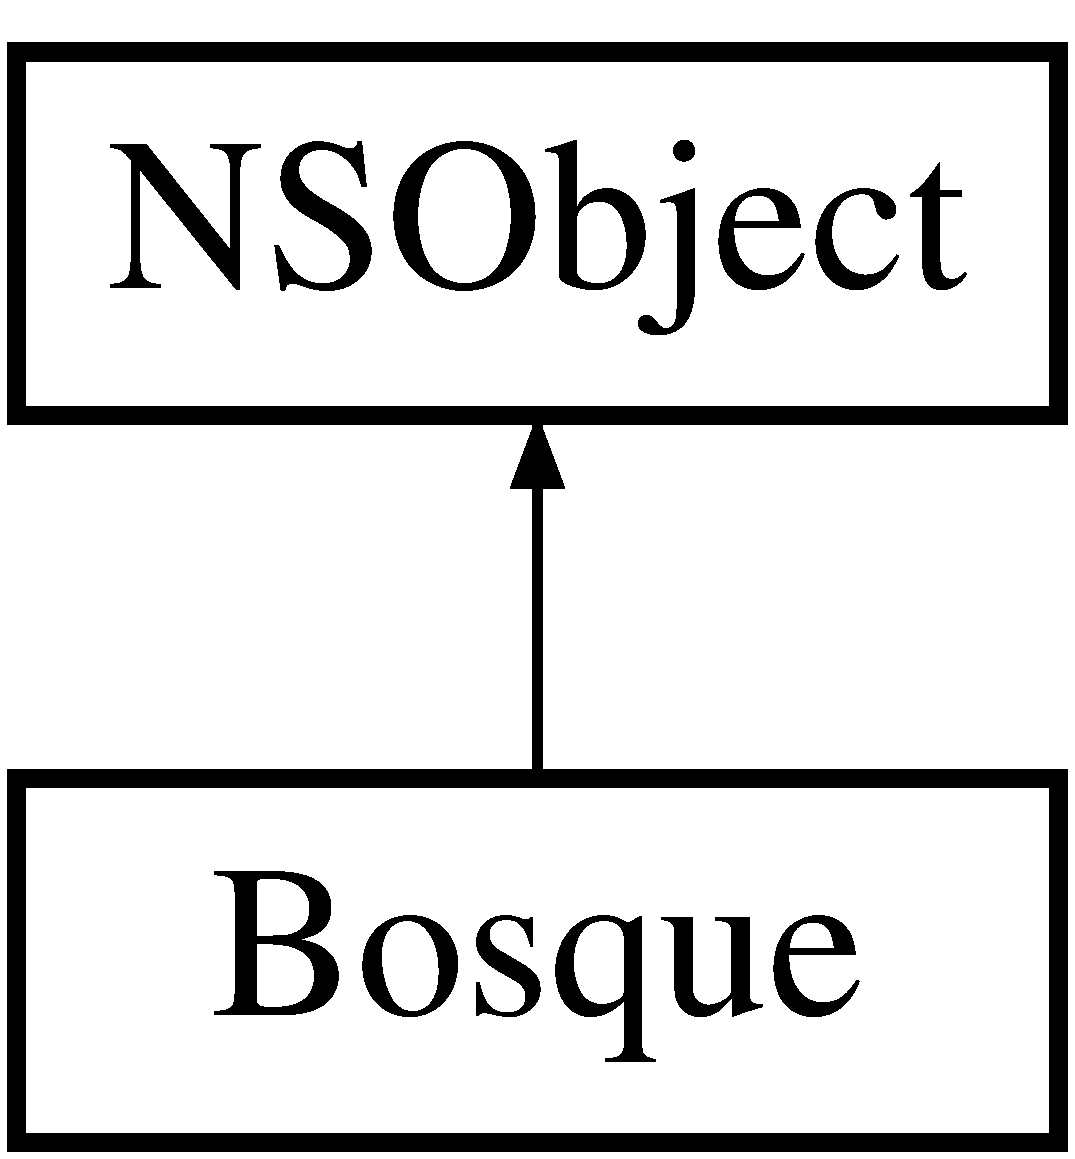
\includegraphics[height=2.000000cm]{interface_bosque}
\end{center}
\end{figure}
\subsection*{Instance Methods}
\begin{DoxyCompactItemize}
\item 
(void) -\/ \hyperlink{interface_bosque_a90cb846dcd7be916917b0990edc11536}{add\+Arvore\+:}
\begin{DoxyCompactList}\small\item\em Adiciona uma árvore na lista de árvores. \end{DoxyCompactList}\item 
(void) -\/ \hyperlink{interface_bosque_a8a118b351cafaf3734fc8c4567cfdb13}{insert\+Arvore\+:posicao\+:}
\begin{DoxyCompactList}\small\item\em Adiciona uma árvore na lista de árvores na posição passada. \end{DoxyCompactList}\item 
(\hyperlink{interface_arvore}{Arvore} $\ast$) -\/ \hyperlink{interface_bosque_a93e40a2af77bbfb6c4ea7a82121645dc}{arvore\+At\+Index\+:}
\item 
(void) -\/ \hyperlink{interface_bosque_a784405d0e2c80b45025157d1206eba7a}{remove\+Arvore\+At\+Index\+:}
\begin{DoxyCompactList}\small\item\em Remove a Árvore que se encontra na posição passada. \end{DoxyCompactList}\end{DoxyCompactItemize}
\subsection*{Properties}
\begin{DoxyCompactItemize}
\item 
N\+S\+Mutable\+Array$<$ \hyperlink{interface_arvore}{Arvore} $\ast$ $>$ $\ast$ \hyperlink{interface_bosque_a4fd04f7b8ff01ab2b7cecb94e4c866f3}{arvores}
\begin{DoxyCompactList}\small\item\em Lista de árvores. \end{DoxyCompactList}\end{DoxyCompactItemize}


\subsection{Detailed Description}
Classe que representa um bosque e suas árvores. 

\subsection{Method Documentation}
\hypertarget{interface_bosque_a90cb846dcd7be916917b0990edc11536}{}\index{Bosque@{Bosque}!add\+Arvore\+:@{add\+Arvore\+:}}
\index{add\+Arvore\+:@{add\+Arvore\+:}!Bosque@{Bosque}}
\subsubsection[{add\+Arvore\+:(\+Arvore $\ast$arvore)}]{\setlength{\rightskip}{0pt plus 5cm}-\/ (void) add\+Arvore\+: 
\begin{DoxyParamCaption}
\item[{({\bf Arvore}$\ast$)}]{arvore}
\end{DoxyParamCaption}
}\label{interface_bosque_a90cb846dcd7be916917b0990edc11536}


Adiciona uma árvore na lista de árvores. 


\begin{DoxyParams}{Parameters}
{\em arvore} & \\
\hline
\end{DoxyParams}
\hypertarget{interface_bosque_a93e40a2af77bbfb6c4ea7a82121645dc}{}\index{Bosque@{Bosque}!arvore\+At\+Index\+:@{arvore\+At\+Index\+:}}
\index{arvore\+At\+Index\+:@{arvore\+At\+Index\+:}!Bosque@{Bosque}}
\subsubsection[{arvore\+At\+Index\+:(int index)}]{\setlength{\rightskip}{0pt plus 5cm}-\/ ({\bf Arvore} $\ast$) arvore\+At\+Index\+: 
\begin{DoxyParamCaption}
\item[{(int)}]{index}
\end{DoxyParamCaption}
}\label{interface_bosque_a93e40a2af77bbfb6c4ea7a82121645dc}
\begin{DoxyReturn}{Returns}
Árvore que se encontra na posição passada. 
\end{DoxyReturn}
\hypertarget{interface_bosque_a8a118b351cafaf3734fc8c4567cfdb13}{}\index{Bosque@{Bosque}!insert\+Arvore\+:posicao\+:@{insert\+Arvore\+:posicao\+:}}
\index{insert\+Arvore\+:posicao\+:@{insert\+Arvore\+:posicao\+:}!Bosque@{Bosque}}
\subsubsection[{insert\+Arvore\+:posicao\+:(\+Arvore $\ast$arvore,[posicao] int index)}]{\setlength{\rightskip}{0pt plus 5cm}-\/ (void) insert\+Arvore\+: 
\begin{DoxyParamCaption}
\item[{({\bf Arvore}$\ast$)}]{arvore}
\item[{posicao:(int)}]{index}
\end{DoxyParamCaption}
}\label{interface_bosque_a8a118b351cafaf3734fc8c4567cfdb13}


Adiciona uma árvore na lista de árvores na posição passada. 


\begin{DoxyParams}{Parameters}
{\em arvore} & \\
\hline
{\em index} & \\
\hline
\end{DoxyParams}
\hypertarget{interface_bosque_a784405d0e2c80b45025157d1206eba7a}{}\index{Bosque@{Bosque}!remove\+Arvore\+At\+Index\+:@{remove\+Arvore\+At\+Index\+:}}
\index{remove\+Arvore\+At\+Index\+:@{remove\+Arvore\+At\+Index\+:}!Bosque@{Bosque}}
\subsubsection[{remove\+Arvore\+At\+Index\+:(int index)}]{\setlength{\rightskip}{0pt plus 5cm}-\/ (void) remove\+Arvore\+At\+Index\+: 
\begin{DoxyParamCaption}
\item[{(int)}]{index}
\end{DoxyParamCaption}
}\label{interface_bosque_a784405d0e2c80b45025157d1206eba7a}


Remove a Árvore que se encontra na posição passada. 



\subsection{Property Documentation}
\hypertarget{interface_bosque_a4fd04f7b8ff01ab2b7cecb94e4c866f3}{}\index{Bosque@{Bosque}!arvores@{arvores}}
\index{arvores@{arvores}!Bosque@{Bosque}}
\subsubsection[{arvores}]{\setlength{\rightskip}{0pt plus 5cm}-\/ (N\+S\+Mutable\+Array$<${\bf Arvore}$\ast$$>$$\ast$) arvores\hspace{0.3cm}{\ttfamily [read]}, {\ttfamily [write]}, {\ttfamily [atomic]}}\label{interface_bosque_a4fd04f7b8ff01ab2b7cecb94e4c866f3}


Lista de árvores. 



The documentation for this class was generated from the following files\+:\begin{DoxyCompactItemize}
\item 
\hyperlink{_bosque_8h}{Bosque.\+h}\item 
\hyperlink{_bosque_8m}{Bosque.\+m}\end{DoxyCompactItemize}

\hypertarget{interface_fruta}{}\section{Fruta Class Reference}
\label{interface_fruta}\index{Fruta@{Fruta}}


classe que representa uma fruta.  




{\ttfamily \#import $<$Fruta.\+h$>$}

Inheritance diagram for Fruta\+:\begin{figure}[H]
\begin{center}
\leavevmode
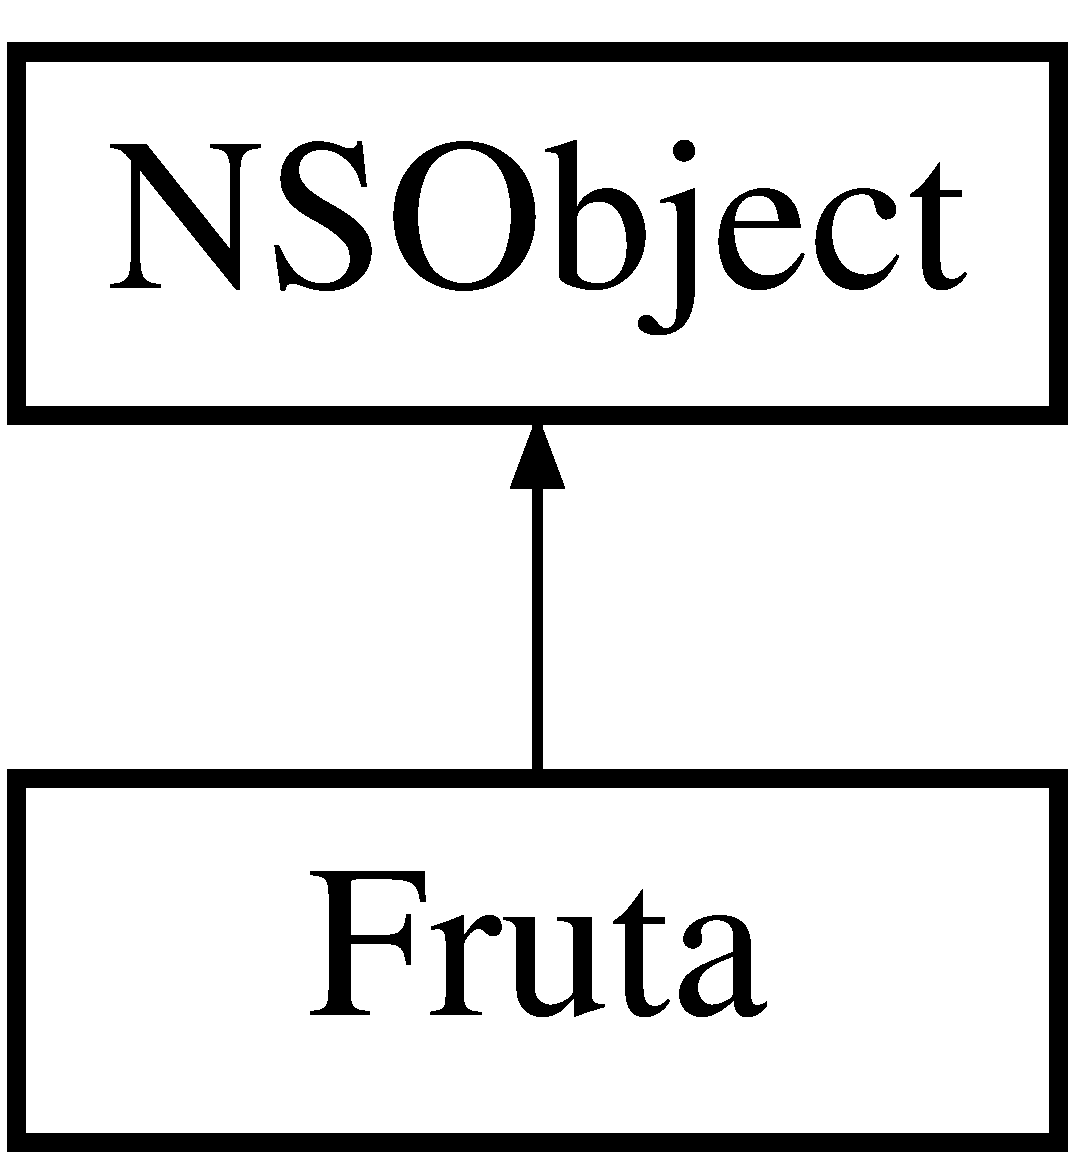
\includegraphics[height=2.000000cm]{interface_fruta}
\end{center}
\end{figure}
\subsection*{Instance Methods}
\begin{DoxyCompactItemize}
\item 
(void) -\/ \hyperlink{interface_fruta_a2cc6d366b344fa39ab64210e18c80f2e}{append\+Analise\+:}
\begin{DoxyCompactList}\small\item\em Adiciona análise da fruta. \end{DoxyCompactList}\item 
(N\+S\+String $\ast$) -\/ \hyperlink{interface_fruta_a41ab1bd0f402fabaf30e0c1b3041a1ea}{get\+Analise}
\end{DoxyCompactItemize}
\subsection*{Properties}
\begin{DoxyCompactItemize}
\item 
N\+S\+Number $\ast$ \hyperlink{interface_fruta_a6bd1235d2a12551a4d02d9885c841539}{nota}
\begin{DoxyCompactList}\small\item\em Nota recebida pela fruta diante da análise da mesma. \end{DoxyCompactList}\item 
N\+S\+Mutable\+String $\ast$ \hyperlink{interface_fruta_a9f497fe605ef82076cac02a5f088f8a5}{analise}
\begin{DoxyCompactList}\small\item\em Análises da fruta. \end{DoxyCompactList}\end{DoxyCompactItemize}


\subsection{Detailed Description}
classe que representa uma fruta. 

\subsection{Method Documentation}
\hypertarget{interface_fruta_a2cc6d366b344fa39ab64210e18c80f2e}{}\index{Fruta@{Fruta}!append\+Analise\+:@{append\+Analise\+:}}
\index{append\+Analise\+:@{append\+Analise\+:}!Fruta@{Fruta}}
\subsubsection[{append\+Analise\+:(\+N\+S\+String $\ast$analise)}]{\setlength{\rightskip}{0pt plus 5cm}-\/ (void) append\+Analise\+: 
\begin{DoxyParamCaption}
\item[{(N\+S\+String$\ast$)}]{analise}
\end{DoxyParamCaption}
}\label{interface_fruta_a2cc6d366b344fa39ab64210e18c80f2e}


Adiciona análise da fruta. 


\begin{DoxyParams}{Parameters}
{\em analise} & \\
\hline
\end{DoxyParams}
\hypertarget{interface_fruta_a41ab1bd0f402fabaf30e0c1b3041a1ea}{}\index{Fruta@{Fruta}!get\+Analise@{get\+Analise}}
\index{get\+Analise@{get\+Analise}!Fruta@{Fruta}}
\subsubsection[{get\+Analise()}]{\setlength{\rightskip}{0pt plus 5cm}-\/ (N\+S\+String $\ast$) get\+Analise 
\begin{DoxyParamCaption}
{}
\end{DoxyParamCaption}
}\label{interface_fruta_a41ab1bd0f402fabaf30e0c1b3041a1ea}
\begin{DoxyReturn}{Returns}
Análise da fruta. 
\end{DoxyReturn}


\subsection{Property Documentation}
\hypertarget{interface_fruta_a9f497fe605ef82076cac02a5f088f8a5}{}\index{Fruta@{Fruta}!analise@{analise}}
\index{analise@{analise}!Fruta@{Fruta}}
\subsubsection[{analise}]{\setlength{\rightskip}{0pt plus 5cm}-\/ (N\+S\+Mutable\+String$\ast$) analise\hspace{0.3cm}{\ttfamily [read]}, {\ttfamily [write]}, {\ttfamily [atomic]}}\label{interface_fruta_a9f497fe605ef82076cac02a5f088f8a5}


Análises da fruta. 

\hypertarget{interface_fruta_a6bd1235d2a12551a4d02d9885c841539}{}\index{Fruta@{Fruta}!nota@{nota}}
\index{nota@{nota}!Fruta@{Fruta}}
\subsubsection[{nota}]{\setlength{\rightskip}{0pt plus 5cm}-\/ (N\+S\+Number$\ast$) nota\hspace{0.3cm}{\ttfamily [read]}, {\ttfamily [write]}, {\ttfamily [atomic]}}\label{interface_fruta_a6bd1235d2a12551a4d02d9885c841539}


Nota recebida pela fruta diante da análise da mesma. 



The documentation for this class was generated from the following files\+:\begin{DoxyCompactItemize}
\item 
\hyperlink{_fruta_8h}{Fruta.\+h}\item 
\hyperlink{_fruta_8m}{Fruta.\+m}\end{DoxyCompactItemize}

\hypertarget{interface_laranjeira}{}\section{Laranjeira Class Reference}
\label{interface_laranjeira}\index{Laranjeira@{Laranjeira}}


Classe que representa uma laranjeira.  




{\ttfamily \#import $<$Laranjeira.\+h$>$}

Inheritance diagram for Laranjeira\+:\begin{figure}[H]
\begin{center}
\leavevmode
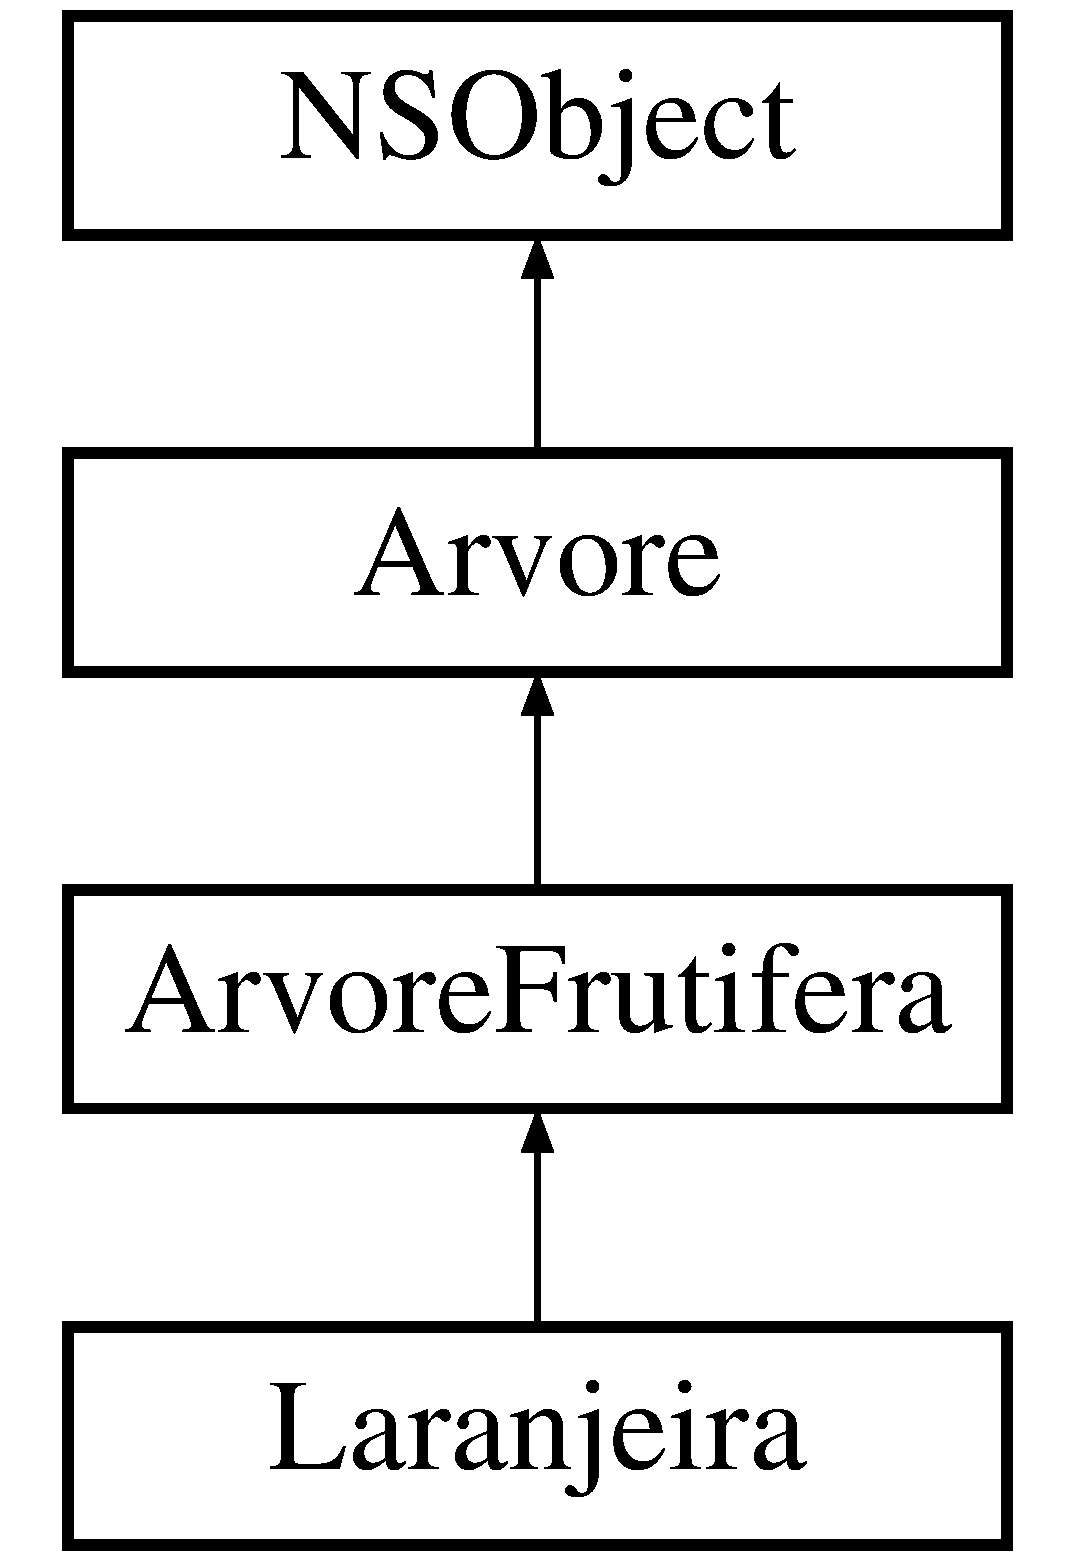
\includegraphics[height=4.000000cm]{interface_laranjeira}
\end{center}
\end{figure}
\subsection*{Instance Methods}
\begin{DoxyCompactItemize}
\item 
(B\+O\+O\+L) -\/ \hyperlink{interface_laranjeira_aaee758b935796457da4d711d7629e6f6}{is\+Laranjeira\+:}
\end{DoxyCompactItemize}
\subsection*{Additional Inherited Members}


\subsection{Detailed Description}
Classe que representa uma laranjeira. 

\subsection{Method Documentation}
\hypertarget{interface_laranjeira_aaee758b935796457da4d711d7629e6f6}{}\index{Laranjeira@{Laranjeira}!is\+Laranjeira\+:@{is\+Laranjeira\+:}}
\index{is\+Laranjeira\+:@{is\+Laranjeira\+:}!Laranjeira@{Laranjeira}}
\subsubsection[{is\+Laranjeira\+:(\+Arvore $\ast$arvore)}]{\setlength{\rightskip}{0pt plus 5cm}-\/ (B\+O\+O\+L) is\+Laranjeira\+: 
\begin{DoxyParamCaption}
\item[{({\bf Arvore}$\ast$)}]{arvore}
\end{DoxyParamCaption}
}\label{interface_laranjeira_aaee758b935796457da4d711d7629e6f6}

\begin{DoxyParams}{Parameters}
{\em arvore} & \\
\hline
\end{DoxyParams}
\begin{DoxyReturn}{Returns}
Flag indicando se a arvore passada é uma laranjeira. 
\end{DoxyReturn}


The documentation for this class was generated from the following files\+:\begin{DoxyCompactItemize}
\item 
\hyperlink{_laranjeira_8h}{Laranjeira.\+h}\item 
\hyperlink{_laranjeira_8m}{Laranjeira.\+m}\end{DoxyCompactItemize}

\hypertarget{interface_limoeiro}{}\section{Limoeiro Class Reference}
\label{interface_limoeiro}\index{Limoeiro@{Limoeiro}}


Classe que representa uma limoeira.  




{\ttfamily \#import $<$Limoeiro.\+h$>$}

Inheritance diagram for Limoeiro\+:\begin{figure}[H]
\begin{center}
\leavevmode
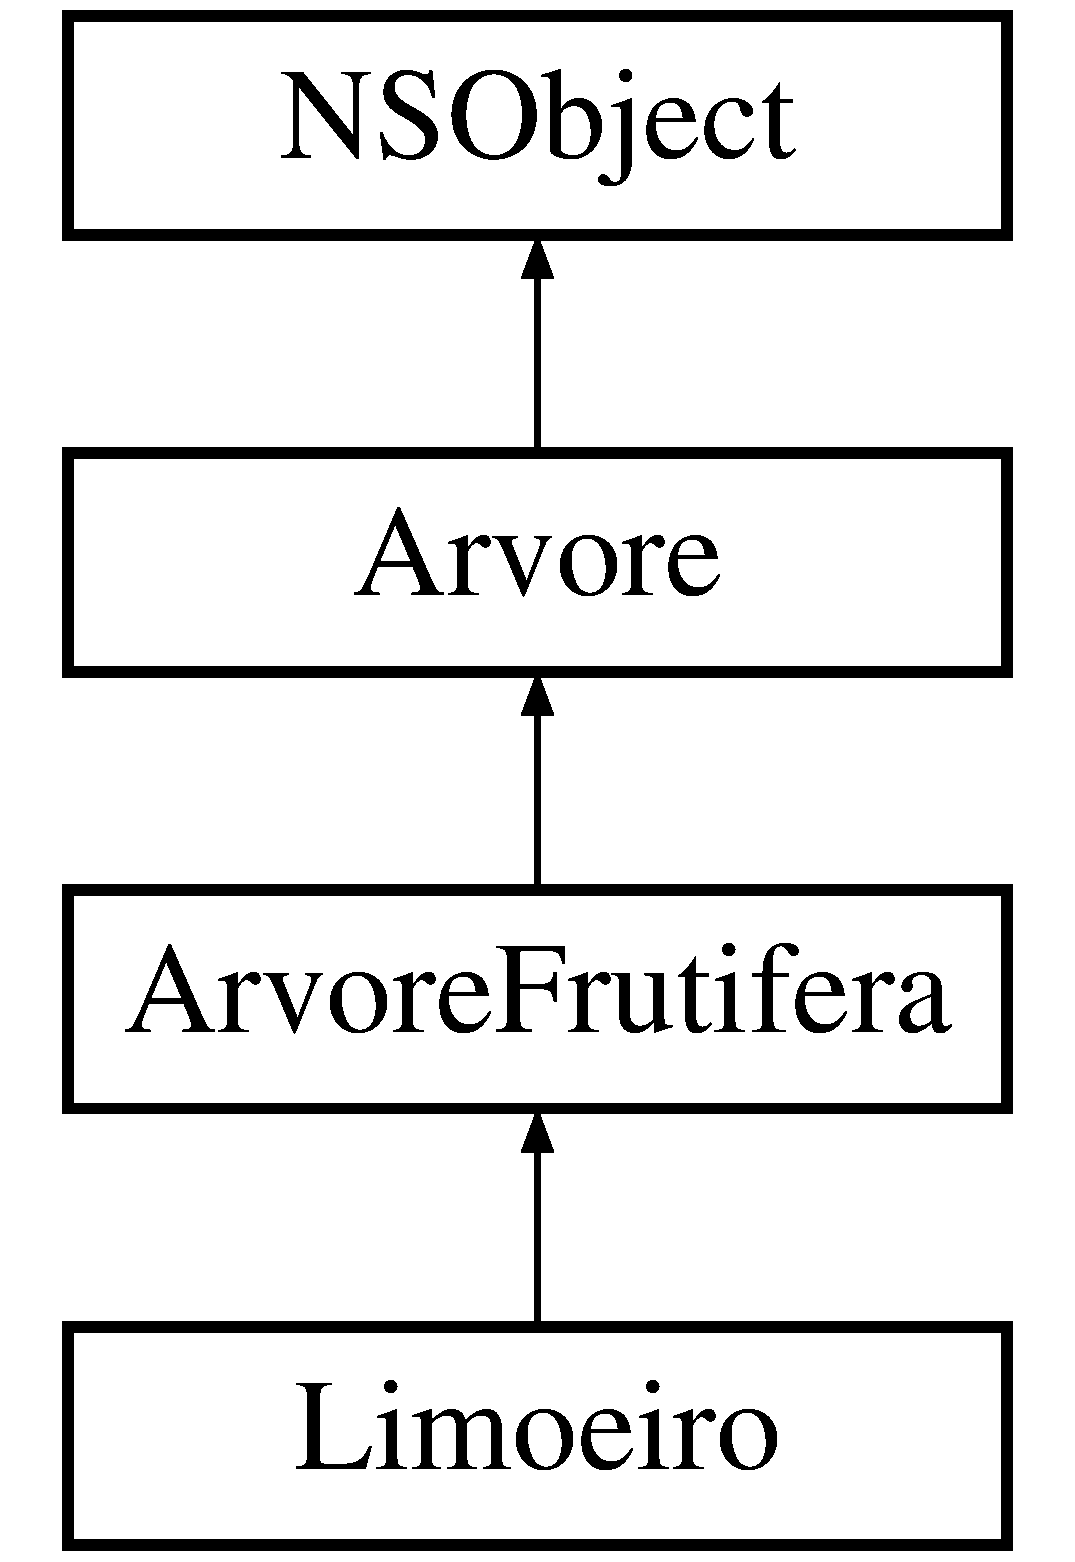
\includegraphics[height=4.000000cm]{interface_limoeiro}
\end{center}
\end{figure}
\subsection*{Instance Methods}
\begin{DoxyCompactItemize}
\item 
(B\+O\+O\+L) -\/ \hyperlink{interface_limoeiro_a589f9e161192981a840035885243f13a}{is\+Limoeiro\+:}
\end{DoxyCompactItemize}
\subsection*{Additional Inherited Members}


\subsection{Detailed Description}
Classe que representa uma limoeira. 

\subsection{Method Documentation}
\hypertarget{interface_limoeiro_a589f9e161192981a840035885243f13a}{}\index{Limoeiro@{Limoeiro}!is\+Limoeiro\+:@{is\+Limoeiro\+:}}
\index{is\+Limoeiro\+:@{is\+Limoeiro\+:}!Limoeiro@{Limoeiro}}
\subsubsection[{is\+Limoeiro\+:(\+Arvore $\ast$arvore)}]{\setlength{\rightskip}{0pt plus 5cm}-\/ (B\+O\+O\+L) is\+Limoeiro\+: 
\begin{DoxyParamCaption}
\item[{({\bf Arvore}$\ast$)}]{arvore}
\end{DoxyParamCaption}
}\label{interface_limoeiro_a589f9e161192981a840035885243f13a}

\begin{DoxyParams}{Parameters}
{\em arvore} & \\
\hline
\end{DoxyParams}
\begin{DoxyReturn}{Returns}
Flag indicando se a arvore passada é um limoeiro. 
\end{DoxyReturn}


The documentation for this class was generated from the following files\+:\begin{DoxyCompactItemize}
\item 
\hyperlink{_limoeiro_8h}{Limoeiro.\+h}\item 
\hyperlink{_limoeiro_8m}{Limoeiro.\+m}\end{DoxyCompactItemize}

\chapter{File Documentation}
\hypertarget{_arvore_8h}{}\section{Arvore.\+h File Reference}
\label{_arvore_8h}\index{Arvore.\+h@{Arvore.\+h}}
{\ttfamily \#import $<$Foundation/\+Foundation.\+h$>$}\\*
\subsection*{Classes}
\begin{DoxyCompactItemize}
\item 
class \hyperlink{interface_arvore}{Arvore}
\begin{DoxyCompactList}\small\item\em Classe que representa uma árvore. \end{DoxyCompactList}\end{DoxyCompactItemize}

\hypertarget{_arvore_8m}{}\section{Arvore.\+m File Reference}
\label{_arvore_8m}\index{Arvore.\+m@{Arvore.\+m}}
{\ttfamily \#import \char`\"{}Arvore.\+h\char`\"{}}\\*

\hypertarget{_arvore_frutifera_8h}{}\section{Arvore\+Frutifera.\+h File Reference}
\label{_arvore_frutifera_8h}\index{Arvore\+Frutifera.\+h@{Arvore\+Frutifera.\+h}}
{\ttfamily \#import \char`\"{}Arvore.\+h\char`\"{}}\\*
{\ttfamily \#import \char`\"{}Fruta.\+h\char`\"{}}\\*
\subsection*{Classes}
\begin{DoxyCompactItemize}
\item 
class \hyperlink{interface_arvore_frutifera}{Arvore\+Frutifera}
\begin{DoxyCompactList}\small\item\em Classe que representa uma árvore frutífera. \end{DoxyCompactList}\end{DoxyCompactItemize}

\hypertarget{_arvore_frutifera_8m}{}\section{Arvore\+Frutifera.\+m File Reference}
\label{_arvore_frutifera_8m}\index{Arvore\+Frutifera.\+m@{Arvore\+Frutifera.\+m}}
{\ttfamily \#import \char`\"{}Arvore\+Frutifera.\+h\char`\"{}}\\*

\hypertarget{_bosque_8h}{}\section{Bosque.\+h File Reference}
\label{_bosque_8h}\index{Bosque.\+h@{Bosque.\+h}}
{\ttfamily \#include $<$Foundation/\+Foundation.\+h$>$}\\*
{\ttfamily \#include \char`\"{}Arvore.\+h\char`\"{}}\\*
\subsection*{Classes}
\begin{DoxyCompactItemize}
\item 
class \hyperlink{interface_bosque}{Bosque}
\begin{DoxyCompactList}\small\item\em Classe que representa um bosque e suas árvores. \end{DoxyCompactList}\end{DoxyCompactItemize}

\hypertarget{_bosque_8m}{}\section{Bosque.\+m File Reference}
\label{_bosque_8m}\index{Bosque.\+m@{Bosque.\+m}}
{\ttfamily \#import \char`\"{}Bosque.\+h\char`\"{}}\\*

\hypertarget{_fruta_8h}{}\section{Fruta.\+h File Reference}
\label{_fruta_8h}\index{Fruta.\+h@{Fruta.\+h}}
{\ttfamily \#include $<$Foundation/\+Foundation.\+h$>$}\\*
\subsection*{Classes}
\begin{DoxyCompactItemize}
\item 
class \hyperlink{interface_fruta}{Fruta}
\begin{DoxyCompactList}\small\item\em classe que representa uma fruta. \end{DoxyCompactList}\end{DoxyCompactItemize}

\hypertarget{_fruta_8m}{}\section{Fruta.\+m File Reference}
\label{_fruta_8m}\index{Fruta.\+m@{Fruta.\+m}}
{\ttfamily \#import \char`\"{}Fruta.\+h\char`\"{}}\\*

\hypertarget{_laranjeira_8h}{}\section{Laranjeira.\+h File Reference}
\label{_laranjeira_8h}\index{Laranjeira.\+h@{Laranjeira.\+h}}
{\ttfamily \#import \char`\"{}Arvore\+Frutifera.\+h\char`\"{}}\\*
\subsection*{Classes}
\begin{DoxyCompactItemize}
\item 
class \hyperlink{interface_laranjeira}{Laranjeira}
\begin{DoxyCompactList}\small\item\em Classe que representa uma laranjeira. \end{DoxyCompactList}\end{DoxyCompactItemize}

\hypertarget{_laranjeira_8m}{}\section{Laranjeira.\+m File Reference}
\label{_laranjeira_8m}\index{Laranjeira.\+m@{Laranjeira.\+m}}
{\ttfamily \#import \char`\"{}Laranjeira.\+h\char`\"{}}\\*

\hypertarget{_limoeiro_8h}{}\section{Limoeiro.\+h File Reference}
\label{_limoeiro_8h}\index{Limoeiro.\+h@{Limoeiro.\+h}}
{\ttfamily \#import \char`\"{}Arvore\+Frutifera.\+h\char`\"{}}\\*
\subsection*{Classes}
\begin{DoxyCompactItemize}
\item 
class \hyperlink{interface_limoeiro}{Limoeiro}
\begin{DoxyCompactList}\small\item\em Classe que representa uma limoeira. \end{DoxyCompactList}\end{DoxyCompactItemize}

\hypertarget{_limoeiro_8m}{}\section{Limoeiro.\+m File Reference}
\label{_limoeiro_8m}\index{Limoeiro.\+m@{Limoeiro.\+m}}
{\ttfamily \#import \char`\"{}Limoeiro.\+h\char`\"{}}\\*

\hypertarget{main_8m}{}\section{main.\+m File Reference}
\label{main_8m}\index{main.\+m@{main.\+m}}
{\ttfamily \#import $<$Foundation/\+Foundation.\+h$>$}\\*
{\ttfamily \#import \char`\"{}Limoeiro.\+h\char`\"{}}\\*
{\ttfamily \#import \char`\"{}Laranjeira.\+h\char`\"{}}\\*
{\ttfamily \#import \char`\"{}Bosque.\+h\char`\"{}}\\*
\subsection*{Functions}
\begin{DoxyCompactItemize}
\item 
int \hyperlink{main_8m_ac0f2228420376f4db7e1274f2b41667c}{main} (int argc, const char $\ast$argv\mbox{[}$\,$\mbox{]})
\end{DoxyCompactItemize}


\subsection{Function Documentation}
\hypertarget{main_8m_ac0f2228420376f4db7e1274f2b41667c}{}\index{main.\+m@{main.\+m}!main@{main}}
\index{main@{main}!main.\+m@{main.\+m}}
\subsubsection[{main(int argc, const char $\ast$argv[])}]{\setlength{\rightskip}{0pt plus 5cm}int main (
\begin{DoxyParamCaption}
\item[{int}]{argc, }
\item[{const char $\ast$}]{argv\mbox{[}$\,$\mbox{]}}
\end{DoxyParamCaption}
)}\label{main_8m_ac0f2228420376f4db7e1274f2b41667c}

%--- End generated contents ---

% Index
\backmatter
\newpage
\phantomsection
\clearemptydoublepage
\addcontentsline{toc}{chapter}{Index}
\printindex

\end{document}
